\documentclass[12pt]{article}
\usepackage[a4paper, portrait, margin=2cm]{geometry}
\usepackage{graphicx} % Required for inserting images
\usepackage[page,toc,titletoc,title]{appendix}
\usepackage{mathptmx}
\usepackage{pdflscape}
\usepackage{pdfpages}
\usepackage{enumitem}
\usepackage{hyperref}
\usepackage{cleveref}
\usepackage{wrapfig}
\usepackage{gensymb}
\usepackage{amssymb}
\usepackage{makecell}
\usepackage{pifont}% http://ctan.org/pkg/pifont
\newcommand{\cmark}{\ding{51}}%
\newcommand{\xmark}{\ding{55}}%

\title{Evaluating The Effectiveness of IDAES and the Ahuora Simulation Platform for Live Data Processing}

\author{Bert Downs\\
\textit{Ahuora Research Group}\\
\textit{University of Waikato}\\
\textit{Hamilton, New Zealand}\\
\texttt{bd65@students.waikato.ac.nz}}

\date{October 2024}

\begin{document}

\maketitle

\section*{Abstract}
% A concise and factual abstract is required. The abstract should state briefly the purpose of the research, the principal results and major conclusions. An abstract is often presented separately from the article, so it must be able to stand alone. For this reason, References should be avoided, but if essential, then cite the author(s) and year(s). Also, non-standard or uncommon abbreviations should be avoided, but if essential they must be defined at their first mention in the abstract itself.

% Keywords. Immediately after the abstract, provide a maximum of 6 keywords avoiding general and plural terms and multiple concepts (avoid, for example, "and", "of"). Be sparing with abbreviations: only abbreviations firmly established in the field may be eligible. These keywords will be used for indexing purposes.


\section{Introduction}
% State the objectives of the work and provide an adequate background, avoiding a detailed literature survey or a summary of the results.

Traditional factory control systems are based on feedback loops that use sensor data to adjust the factory's state. However, these systems are limited in their ability to predict future states and optimise factory performance. Digital Twinning is a new approach that combines live factory data, historical state, mathematical modelling, and data-driven modelling to create a digital replica of the factory. 
However, in existing literature, most examples of digital twinning focus on specific situations, rather than providing a general framework for creating digital twins. Many remain at the proof-of-concept stage, and have not yet been deployed in industrial settings.

In order to implement digital twinning in industry, simulation platforms must be able to work with and process live data, but most simulation environments are designed for design and analysis, rather than real-time processing \cite{agi2024computational}. The objective of this research is to evaluate how effectively an existing simulation platform can be used or extended to process live data.

One such simulation platform is the IDAES-PSE\footnote{IDAES: Institute for the Design of Advanced Energy Systems - Process Simulation Environment, \href{https://idaes-pse.readthedocs.io}{https://idaes-pse.readthedocs.io}} modelling framework, which is designed for the analysis of chemical processes \cite{lee2021idaes}. It supports a variety of modelling techniques, including steady-state chemical modelling, and dynamic modelling of time-dependent processes. 
It has also been extended to support data-driven modelling techniques, using libraries such as PySMO\footnote{PySMO: Python-based Surrogate Modelling Objects, \href{https://idaes-pse.readthedocs.io/en/stable/explanations/modeling_extensions/surrogate/api/pysmo/index.html}{https://idaes-pse.readthedocs.io}} and OMLT\footnote{OMLT: Optimization and Machine Learning Toolkit, \href{https://omlt.readthedocs.io/en/latest/}{https://omlt.readthedocs.io/en/latest/}} \cite{cecconOMLTOptimizationMachine2022} 

This research evaluates the extent to which the IDAES-PSE modelling framework can be used to implement emerging chemical modelling techniques for live data processing, to prove it's suitability as a platform on which to develop such tools.

\section{Method}
%Experimental procedure
%Provide sufficient details to allow the work to be reproduced by an independent researcher. Methods that are already published should be summarized, and indicated by a reference. If quoting directly from a previously published method, use quotation marks and also cite the source. Any modifications to existing methods should also be described.
%This section can contain Material and methods and Theory/calculation. A Theory section should extend, not repeat, the background to the article already dealt with in the Introduction and lay the foundation for further work. In contrast, a Calculation section represents a practical development from a theoretical basis.

IDAES has many components, so an iterative validation process is used. The evaluation is broken down into parts, each focusing on a different piece of functionality. 

The core functionality of the IDAES modelling framework is steady-state modelling, where a chemical system is in a stable equilibrium and variables do not change over time. In a live data processing context, steady-state simulations can be used to model the entire state of the factory, based on a sample of avaliable sensor data. Multiple steady-state simulations can be run at different time steps, but each represents a stable equilibrium. This is the simplest form of modelling to integrate with live data. 

\begin{table}[h]
    \centering
    \begin{tabular}{|l|p{10cm}|}
        \hline
        \textbf{Functionality} & \textbf{Description} \\
        \hline
        Steady State Modelling & Analysis of systems in a stable equilibrium where variables do not change over time. \\
        \hline
        Dynamics & Modelling of time-dependent processes to understand how systems evolve over time. \\
        \hline
        Optimisation/Control & Techniques to find the best operating conditions or control strategies for a system. \\
        \hline
        Hybrid Modelling & Combining different modelling approaches, such as data-driven and first-principles models, to improve accuracy and robustness. \\
        \hline
    \end{tabular}
    \caption{Different pieces of functionality evaluated from the IDAES-PSE framework.}
    \label{tab:functionality}
\end{table}

Dynamic Modelling adds a time dimension to the simulation, allowing changes in the system to propogate through over time. This is useful for predicting how a factory will respond to changes in input conditions, and can be a key decision-making tool for factory operators.

Optimisation and Control techniques can be used to find the best operating conditions for a system, or to develop control strategies that keep the system in a desired state. This enables closed-loop control of a industrial process, where the system can automatically adjust itself to maintain optimal conditions.

Hybrid Modelling implements Machine Learning techniques into the model. IDAES is built on Pyomo, an algebraic modelling language \cite{bynum2021pyomo}, but it is possible to combine machine learning techniques with data-driven modelling libraries such as PySMO. 
This is useful for situations where the system is too complex to model using a single approach, or where data is available but the underlying physics are not well understood for parts of the system. 
The aim of hybrid modelling is to increase generalisation and explainability compared to purely data-driven models, and increase accuracy and adaptability compared to purely first-principles models.

\subsection{Evaluation Criteria}

Each functionality is tested using by developing and evaluating a simple prototype in the IDAES-PSE framework. The methodology for evaluation is akin to industry acceptance testing, where the prototype is tested against a set of requirements to determine if it meets each of them or not. 


\begin{table}[h]
    \centering
    \begin{tabular}{|l|p{10cm}|}
        \hline
        \textbf{Criteria} & \textbf{Description} \\
        \hline
        Completeness as a Standalone Tool & Evaluates how complete (stable, developed, documented, robust) the functionality is, without any consideration for live data. \\
        \hline
        Ease of Integration & Measures how easily the framework can be integrated with existing systems and workflows, including compatibility with other software and data formats. \\
        \hline
        Suitability for Live Data Processing & Assesses how easily the functionality could be used in a real-time data processing scenario, assuming tooling was added for data ingestion and output. \\
        \hline
    \end{tabular}
    \caption{Evaluation criteria for the IDAES-PSE framework.}
    \label{tab:evaluation_criteria}
\end{table}


The evaluation criteria do not focus on the accuracy of the IDAES platform in performing chemical simulations, or user-friendliness of the interfaces, or the performance of the solving process itself. Those characteristics are considered out of scope of this study, and are evaluated elsewhere \cite{hart2011pyomo} \cite{myhre2022investigation}. Instead, the evaluation criteria focus on the ability of the IDAES platform to be used for live data processing, and the ease of integration with other systems.

% TODO: Why these evaluation criteria?
``Completeness as a Standalone Tool'' is the first criteria for evaluation. It is important because it provides a baseline for the other criteria. If the functionality is not complete as a standalone tool, then it is unlikely to be useful for live data processing. 

``Ease of Integration'' is chosen as the second criteria for evaluation. This is because to be useful in industry, it must be possible to integrate the functionality in IDAES with existing systems for model development and data processing.

``Suitability for Live Data Processing'' is chosen as the final criteria. It is the most high-level, and to some degree it builds on the other two. However, it also considers the application of the functionality in a real-world system, and whether or not the functionality is useful in an online environment.

The source code of each prototype is avaliable on Github\footnote{\href{https://github.com/bertkdowns/model-predictive-control}{https://github.com/bertkdowns/model-predictive-control}}.

% Max 1 page per functionality evaluated.
\section{Steady State Modelling}

% Explain what you did to analyse it

\subsection{Test Case}

A heat pump model is built in IDAES to simulate the steady-state operation of a heat pump dryer. The model is based on a simple heat pump cycle, where a refrigerant is compressed, condensed, expanded, and evaporated to transfer heat from one side of the system to the other. This can be solved at steady state to determine the operating conditions of the heat pump, such as the temperature and pressure of the refrigerant at each stage of the cycle.

% explain how it works internally - e.g pyomo sets, variables, constraints, etc
% ideaes hides a lot of the complexity but in a good way

\subsection{Evaluation}

% explain why it is/isnt complete as a standalone tool
This tests the core functionality of IDAES. Developing this type of model is well-documented and supported, and solving is robust as long as the model is built with physically feasible conditions.

% explain why it is/isnt easy to integrate with other systems
IDAES is based on Pyomo, and multi-steady-state simulations only use the core Pyomo functionality. This makes it easy to integrate with other systems that use Pyomo. However, tools from other algebraic modelling languages would require additional work to integrate. Pyomo's ecosystem is large enough that it can be considered to be well-supported.

% explain why it is/isnt suitable for live data processing

To use this in a live simulation context, the model would need to be re-solved at regular intervals, with new sensor data being used to update the model. Sensor data could be used to update the model's parameters, and Pyomo allows creating additional constraints to map sensor data to model parameters. It would be possible to use a steady-state idaes model in a live data processing context, if it was integrated into a process toolchain.


\section{Dynamics} \label{sec:dynamics}


\subsection{Test Case}
% Explain what you did to analyse it

To evaluate dynamics, a model of a steam tank, with a valve controlling the inlet and outlet pressure and flow rate, is created. A PID controller is used to control the valve opening fraction to regulate the pressure in the tank.

\begin{figure}
    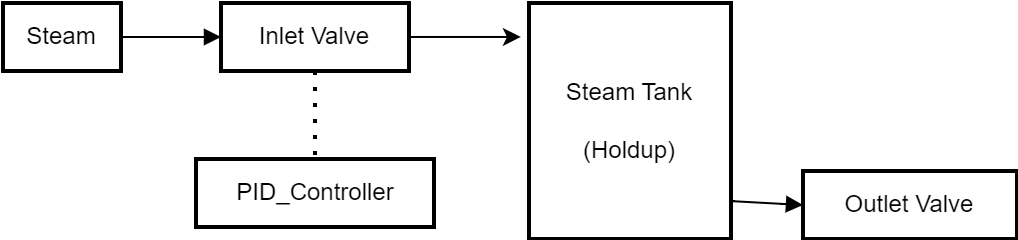
\includegraphics[width=0.9\textwidth]{../dynamicmodelling.png}
    \caption{Dynamic Modelling of a Steam Tank}
    \label{fig:dynamicmodelling}
\end{figure}

This provides a simple example of a dynamic system. The inlet and outlet valve and the PID controller were not dynamic models: From a mathematical perspective, this means their properties were fully determined by the inlet and outlet conditions. The only dynamic model in this flowsheet is the Steam Tank. From a mathematical perspective, this means that the state of the steam tank is determined by the inlet and outlet conditions, but also the previous state of the tank, i.e how ``full" the tank is. In chemical engineering, this is often referred to as the ``holdup" of the tank.

% todo: discuss how it actually does this: pyomo differentiation, sets, timescales, etc

The dynamic functionality of IDAES is built on the library Pyomo.DAE \cite{nicholson2018pyomo}, which allows for the creation and solution of differential algebraic equations. It extends Pyomo to support a ContinuousSet, or bounded continuous domain, over which derivatives and integrals can be calculated. 

Internally, Pyomo.DAE breaks the continuous domain into a series of finite time steps. Thus, constraints to the IDAES model are specified as a function of time, which is discretised and evaluated at each time step.

To test this, a dynamic model was created, and constraints were used to model a ramp in inlet pressure over time. This was done by specifying an equation for the inlet pressure,to be applied at each time step

\subsection{Evaluation}
% explain why it is/isnt complete as a standalone tool
The IDAES framework is well-suited to dynamic modelling, as it provides tools for creating and solving differential equations. It can easily model the same system at different time scales. Dynamic models certainly are much more complex than steady-state models, but IDAES and Pyomo provide the tools to handle this complexity.

% explain why it is/isnt easy to integrate with other systems
Extracting data and setting properties for a dynamic model is much the same as for a steady-state model, as it uses similar Pyomo constructs. Because the dynamic model is broken down into algebraic equations, it can be solved in the same way as a steady state simulation. Simple idaes flowsheets can easily be extended to include dynamic models, and the same tools can be used to solve them. 

% explain why it is/isnt suitable for live data processing
Dynamic models can be used in two different ways for live data processing. First, the initial conditions of the model can be specified from live data, and then the dynamic model can be solved to predict future states. If the model and initial conditions are specified correctly, from a software development perspective this is no more complex than a steady state model (even though it is much more complex as a mathematical or chemical system), as the same data attributes need to be accessed. 

Alternatively, constraint functions (such as in the test case) could be generated from the live data so that the model simulates the real-world changes in variables. Sensor data is not a continuous domain, so an interpolation or modelling strategy would need to be created to handle this. The tools of Pyomo.DAE are flexible enough to allow for this, so dynamic modelling in IDAES would be suitable in a live data processing context.

\section{Optimisation/Control}

\subsection{Test Case}

% Explain what you did to analyse it - the test case
To analyse optimisation, a hydrodealkylation (HDA) reaction model is evaluated. The source code for this model is avaliable in the IDAES examples documentation\footnote{\href{https://idaes.github.io/examples-pse/latest/Tutorials/Basics/HDA_flowsheet_solution_doc.html}{https://idaes.github.io/examples-pse/latest/Tutorials/Basics/HDA\_flowsheet\_solution\_doc.html}}.

To optimise the flowsheet, firstly the model is solved as a square problem (with all values specified). This enables getting a good initial location to start optimising from.
Then, variables are unfixed to create a space to optimise over, and an objective function is added to the model.

Pyomo natively supports objective functions, that the optimization solver attempts to maximise or minimise. They are specified as an expression, in a similar way to constraints. In the HDA test case, the objective function is to minimise the operating cost, which is a function of the total heating and cooling costs of the system. 

To analyse control, the IDAES Caprese \footnote{\href{https://idaes-pse.readthedocs.io/en/stable/explanations/modeling_extensions/caprese/nmpc.html}{https://idaes-pse.readthedocs.io/en/stable/explanations/modeling\_extensions/caprese/nmpc.html}} library was investigated. Caprese supports simulating model predictive control, where plant inputs are determined by solving an optimisation problem at each time step. However, it can only simulate control, and thus would not be an appropriate tool for use in a live data pipeline.

Other than model predictive control, there is little support for optimising dynamic flowsheets in IDAES. The methods that do exist use surrogate models, to linearise the problem. Surrogate models will be discussed \cref{sec:hybrid}.

% explain how it works internally


\subsection{Evaluation}
% explain why it is/isnt complete as a standalone tool

Because optimisation has first-party support from Pyomo, and because creating optimisation functions is

% explain why it is/isnt easy to integrate with other systems

% explain why it is/isnt suitable for live data processing
\section{Hybrid Modelling} \label{sec:hybrid}
\subsection{Test Case}

% Explain what you did to analyse it - the test case

To test the workflow for hybrid modelling, a simple surrogate model is created using PySMO. First, a set of data points is generated by solving a valve model at different pressures, temperatures, and flow rates. Then, this data is used to train a surrogate model, which can predict the outlet pressure and enthalpy from the valve based on the inlet conditions. This generated data for a steady-state simulation, 

The weights of the trained model are then saved to disk. 

% TODO: Add a screenshot of appending the data points to create the flowsheet
% also add a screenshot of creating the surrogate model with the data points
% and maybe a graph of the data vs the surrogate model at predicting things

% explain how it works internally


\subsection{Evaluation}

% explain why it is/isnt complete as a standalone tool

% explain why it is/isnt easy to integrate with other systems

% explain why it is/isnt suitable for live data processing

\section{Results \& Discussion}
%Results should be clear and concise.

% TODO: Add a table for each piece of functionality evaluated, showing the results of the evaluation against the criteria.

\begin{table}[h]
    \centering
    \begin{tabular}{|l|p{0.2\textwidth}|p{0.2\textwidth}|p{0.21\textwidth}|}
        \hline
        \textbf{Functionality} & \textbf{Completeness as a Standalone Tool} & \textbf{Ease of Integration} & \textbf{Suitability for Live Data Processing} \\
        \hline
        Steady State Modelling & \hfil \cmark & \hfil \cmark & \hfil \cmark \\ \hline
        Dynamics & \hfil \cmark & \hfil \cmark  & \makecell{\cmark \\\footnotesize{(if specified correctly)} } \\\hline
        Optimisation/Control & \makecell{\cmark \\\footnotesize{(via pyomo)} } & \hfil \cmark & \makecell{ \footnotesize{Needs platform} \\\footnotesize{for control}} \\\hline
        Hybrid Modelling & \hfil \cmark & \makecell{ \footnotesize{Only focused on }\\\footnotesize{batch learning}} & \makecell{\cmark \\\footnotesize{(except dynamic models)} } \\
        \hline
    \end{tabular}
    \caption{Evaluation of IDAES-PSE functionality against the criteria.}
    \label{tab:results}
\end{table}

% Discussion
% This should explore the significance of the results of the work, not repeat them. A combined Results and Discussion section is often appropriate. Avoid extensive citations and discussion of published literature.
%Note: results and Discussion can also be combined in a single section.


\section{Conclusions}
% The main conclusions of the study may be presented in a short Conclusions section, which may stand alone or form a subsection of a Discussion or Results and Discussion section.


\section*{Acknowledgements}
% Collate acknowledgements in a separate section at the end of the article before the references and do not, therefore, include them on the title page, as a footnote to the title or otherwise. List here those individuals who provided help during the research (e.g., providing language help, writing assistance or proof reading the article, etc.).



% References
% Please ensure that every reference cited in the text is also present in the reference list (and vice versa). Unpublished results and personal communications are not recommended in the reference list, but may be mentioned in the text. If these references are included in the reference list they should follow the standard reference style.
\bibliographystyle{apalike}
\bibliography{refs} % Entries are in the refs.bib file



% If there is more than one appendix, they should be identified as A, B, etc. Formulae and equations in appendices should be given separate numbering: Eq. (A.1), Eq. (A.2), etc.; in a subsequent appendix, Eq. (B.1) and so on. Similarly for tables and figures: Table A.1; Fig. A.1, etc.
\begin{appendices}


\end{appendices}


\end{document}